% Options for packages loaded elsewhere
\PassOptionsToPackage{unicode}{hyperref}
\PassOptionsToPackage{hyphens}{url}
\PassOptionsToPackage{dvipsnames,svgnames,x11names}{xcolor}
%
\documentclass[
  letterpaper,
  DIV=11,
  numbers=noendperiod]{scrartcl}

\usepackage{amsmath,amssymb}
\usepackage{lmodern}
\usepackage{iftex}
\ifPDFTeX
  \usepackage[T1]{fontenc}
  \usepackage[utf8]{inputenc}
  \usepackage{textcomp} % provide euro and other symbols
\else % if luatex or xetex
  \usepackage{unicode-math}
  \defaultfontfeatures{Scale=MatchLowercase}
  \defaultfontfeatures[\rmfamily]{Ligatures=TeX,Scale=1}
\fi
% Use upquote if available, for straight quotes in verbatim environments
\IfFileExists{upquote.sty}{\usepackage{upquote}}{}
\IfFileExists{microtype.sty}{% use microtype if available
  \usepackage[]{microtype}
  \UseMicrotypeSet[protrusion]{basicmath} % disable protrusion for tt fonts
}{}
\makeatletter
\@ifundefined{KOMAClassName}{% if non-KOMA class
  \IfFileExists{parskip.sty}{%
    \usepackage{parskip}
  }{% else
    \setlength{\parindent}{0pt}
    \setlength{\parskip}{6pt plus 2pt minus 1pt}}
}{% if KOMA class
  \KOMAoptions{parskip=half}}
\makeatother
\usepackage{xcolor}
\setlength{\emergencystretch}{3em} % prevent overfull lines
\setcounter{secnumdepth}{-\maxdimen} % remove section numbering
% Make \paragraph and \subparagraph free-standing
\ifx\paragraph\undefined\else
  \let\oldparagraph\paragraph
  \renewcommand{\paragraph}[1]{\oldparagraph{#1}\mbox{}}
\fi
\ifx\subparagraph\undefined\else
  \let\oldsubparagraph\subparagraph
  \renewcommand{\subparagraph}[1]{\oldsubparagraph{#1}\mbox{}}
\fi

\usepackage{color}
\usepackage{fancyvrb}
\newcommand{\VerbBar}{|}
\newcommand{\VERB}{\Verb[commandchars=\\\{\}]}
\DefineVerbatimEnvironment{Highlighting}{Verbatim}{commandchars=\\\{\}}
% Add ',fontsize=\small' for more characters per line
\usepackage{framed}
\definecolor{shadecolor}{RGB}{241,243,245}
\newenvironment{Shaded}{\begin{snugshade}}{\end{snugshade}}
\newcommand{\AlertTok}[1]{\textcolor[rgb]{0.68,0.00,0.00}{#1}}
\newcommand{\AnnotationTok}[1]{\textcolor[rgb]{0.37,0.37,0.37}{#1}}
\newcommand{\AttributeTok}[1]{\textcolor[rgb]{0.40,0.45,0.13}{#1}}
\newcommand{\BaseNTok}[1]{\textcolor[rgb]{0.68,0.00,0.00}{#1}}
\newcommand{\BuiltInTok}[1]{\textcolor[rgb]{0.00,0.23,0.31}{#1}}
\newcommand{\CharTok}[1]{\textcolor[rgb]{0.13,0.47,0.30}{#1}}
\newcommand{\CommentTok}[1]{\textcolor[rgb]{0.37,0.37,0.37}{#1}}
\newcommand{\CommentVarTok}[1]{\textcolor[rgb]{0.37,0.37,0.37}{\textit{#1}}}
\newcommand{\ConstantTok}[1]{\textcolor[rgb]{0.56,0.35,0.01}{#1}}
\newcommand{\ControlFlowTok}[1]{\textcolor[rgb]{0.00,0.23,0.31}{#1}}
\newcommand{\DataTypeTok}[1]{\textcolor[rgb]{0.68,0.00,0.00}{#1}}
\newcommand{\DecValTok}[1]{\textcolor[rgb]{0.68,0.00,0.00}{#1}}
\newcommand{\DocumentationTok}[1]{\textcolor[rgb]{0.37,0.37,0.37}{\textit{#1}}}
\newcommand{\ErrorTok}[1]{\textcolor[rgb]{0.68,0.00,0.00}{#1}}
\newcommand{\ExtensionTok}[1]{\textcolor[rgb]{0.00,0.23,0.31}{#1}}
\newcommand{\FloatTok}[1]{\textcolor[rgb]{0.68,0.00,0.00}{#1}}
\newcommand{\FunctionTok}[1]{\textcolor[rgb]{0.28,0.35,0.67}{#1}}
\newcommand{\ImportTok}[1]{\textcolor[rgb]{0.00,0.46,0.62}{#1}}
\newcommand{\InformationTok}[1]{\textcolor[rgb]{0.37,0.37,0.37}{#1}}
\newcommand{\KeywordTok}[1]{\textcolor[rgb]{0.00,0.23,0.31}{#1}}
\newcommand{\NormalTok}[1]{\textcolor[rgb]{0.00,0.23,0.31}{#1}}
\newcommand{\OperatorTok}[1]{\textcolor[rgb]{0.37,0.37,0.37}{#1}}
\newcommand{\OtherTok}[1]{\textcolor[rgb]{0.00,0.23,0.31}{#1}}
\newcommand{\PreprocessorTok}[1]{\textcolor[rgb]{0.68,0.00,0.00}{#1}}
\newcommand{\RegionMarkerTok}[1]{\textcolor[rgb]{0.00,0.23,0.31}{#1}}
\newcommand{\SpecialCharTok}[1]{\textcolor[rgb]{0.37,0.37,0.37}{#1}}
\newcommand{\SpecialStringTok}[1]{\textcolor[rgb]{0.13,0.47,0.30}{#1}}
\newcommand{\StringTok}[1]{\textcolor[rgb]{0.13,0.47,0.30}{#1}}
\newcommand{\VariableTok}[1]{\textcolor[rgb]{0.07,0.07,0.07}{#1}}
\newcommand{\VerbatimStringTok}[1]{\textcolor[rgb]{0.13,0.47,0.30}{#1}}
\newcommand{\WarningTok}[1]{\textcolor[rgb]{0.37,0.37,0.37}{\textit{#1}}}

\providecommand{\tightlist}{%
  \setlength{\itemsep}{0pt}\setlength{\parskip}{0pt}}\usepackage{longtable,booktabs,array}
\usepackage{calc} % for calculating minipage widths
% Correct order of tables after \paragraph or \subparagraph
\usepackage{etoolbox}
\makeatletter
\patchcmd\longtable{\par}{\if@noskipsec\mbox{}\fi\par}{}{}
\makeatother
% Allow footnotes in longtable head/foot
\IfFileExists{footnotehyper.sty}{\usepackage{footnotehyper}}{\usepackage{footnote}}
\makesavenoteenv{longtable}
\usepackage{graphicx}
\makeatletter
\def\maxwidth{\ifdim\Gin@nat@width>\linewidth\linewidth\else\Gin@nat@width\fi}
\def\maxheight{\ifdim\Gin@nat@height>\textheight\textheight\else\Gin@nat@height\fi}
\makeatother
% Scale images if necessary, so that they will not overflow the page
% margins by default, and it is still possible to overwrite the defaults
% using explicit options in \includegraphics[width, height, ...]{}
\setkeys{Gin}{width=\maxwidth,height=\maxheight,keepaspectratio}
% Set default figure placement to htbp
\makeatletter
\def\fps@figure{htbp}
\makeatother

\usepackage{booktabs}
\usepackage{longtable}
\usepackage{array}
\usepackage{multirow}
\usepackage{wrapfig}
\usepackage{float}
\usepackage{colortbl}
\usepackage{pdflscape}
\usepackage{tabu}
\usepackage{threeparttable}
\usepackage{threeparttablex}
\usepackage[normalem]{ulem}
\usepackage{makecell}
\usepackage{xcolor}
\KOMAoption{captions}{tableheading}
\makeatletter
\@ifpackageloaded{tcolorbox}{}{\usepackage[many]{tcolorbox}}
\@ifpackageloaded{fontawesome5}{}{\usepackage{fontawesome5}}
\definecolor{quarto-callout-color}{HTML}{909090}
\definecolor{quarto-callout-note-color}{HTML}{0758E5}
\definecolor{quarto-callout-important-color}{HTML}{CC1914}
\definecolor{quarto-callout-warning-color}{HTML}{EB9113}
\definecolor{quarto-callout-tip-color}{HTML}{00A047}
\definecolor{quarto-callout-caution-color}{HTML}{FC5300}
\definecolor{quarto-callout-color-frame}{HTML}{acacac}
\definecolor{quarto-callout-note-color-frame}{HTML}{4582ec}
\definecolor{quarto-callout-important-color-frame}{HTML}{d9534f}
\definecolor{quarto-callout-warning-color-frame}{HTML}{f0ad4e}
\definecolor{quarto-callout-tip-color-frame}{HTML}{02b875}
\definecolor{quarto-callout-caution-color-frame}{HTML}{fd7e14}
\makeatother
\makeatletter
\makeatother
\makeatletter
\makeatother
\makeatletter
\@ifpackageloaded{caption}{}{\usepackage{caption}}
\AtBeginDocument{%
\ifdefined\contentsname
  \renewcommand*\contentsname{Table of contents}
\else
  \newcommand\contentsname{Table of contents}
\fi
\ifdefined\listfigurename
  \renewcommand*\listfigurename{List of Figures}
\else
  \newcommand\listfigurename{List of Figures}
\fi
\ifdefined\listtablename
  \renewcommand*\listtablename{List of Tables}
\else
  \newcommand\listtablename{List of Tables}
\fi
\ifdefined\figurename
  \renewcommand*\figurename{Figure}
\else
  \newcommand\figurename{Figure}
\fi
\ifdefined\tablename
  \renewcommand*\tablename{Table}
\else
  \newcommand\tablename{Table}
\fi
}
\@ifpackageloaded{float}{}{\usepackage{float}}
\floatstyle{ruled}
\@ifundefined{c@chapter}{\newfloat{codelisting}{h}{lop}}{\newfloat{codelisting}{h}{lop}[chapter]}
\floatname{codelisting}{Listing}
\newcommand*\listoflistings{\listof{codelisting}{List of Listings}}
\makeatother
\makeatletter
\@ifpackageloaded{caption}{}{\usepackage{caption}}
\@ifpackageloaded{subcaption}{}{\usepackage{subcaption}}
\makeatother
\makeatletter
\@ifpackageloaded{tcolorbox}{}{\usepackage[many]{tcolorbox}}
\makeatother
\makeatletter
\@ifundefined{shadecolor}{\definecolor{shadecolor}{rgb}{.97, .97, .97}}
\makeatother
\makeatletter
\makeatother
\ifLuaTeX
  \usepackage{selnolig}  % disable illegal ligatures
\fi
\IfFileExists{bookmark.sty}{\usepackage{bookmark}}{\usepackage{hyperref}}
\IfFileExists{xurl.sty}{\usepackage{xurl}}{} % add URL line breaks if available
\urlstyle{same} % disable monospaced font for URLs
\hypersetup{
  pdftitle={Weekly 5 Summary},
  pdfauthor={Gaurang Kakade},
  colorlinks=true,
  linkcolor={blue},
  filecolor={Maroon},
  citecolor={Blue},
  urlcolor={Blue},
  pdfcreator={LaTeX via pandoc}}

\title{Weekly 5 Summary}
\author{Gaurang Kakade}
\date{}

\begin{document}
\maketitle
\ifdefined\Shaded\renewenvironment{Shaded}{\begin{tcolorbox}[sharp corners, frame hidden, breakable, borderline west={3pt}{0pt}{shadecolor}, enhanced, boxrule=0pt, interior hidden]}{\end{tcolorbox}}\fi

\renewcommand*\contentsname{Table of contents}
{
\hypersetup{linkcolor=}
\setcounter{tocdepth}{3}
\tableofcontents
}
\begin{center}\rule{0.5\linewidth}{0.5pt}\end{center}

\hypertarget{tuesday-feb-7}{%
\subsection{Tuesday, Feb 7}\label{tuesday-feb-7}}

\begin{tcolorbox}[enhanced jigsaw, bottomrule=.15mm, coltitle=black, breakable, opacityback=0, rightrule=.15mm, colframe=quarto-callout-important-color-frame, toptitle=1mm, leftrule=.75mm, opacitybacktitle=0.6, bottomtitle=1mm, titlerule=0mm, title=\textcolor{quarto-callout-important-color}{\faExclamation}\hspace{0.5em}{TIL}, arc=.35mm, toprule=.15mm, colbacktitle=quarto-callout-important-color!10!white, colback=white, left=2mm]

Today, I learnt the following concepts in class:

\begin{enumerate}
\def\labelenumi{\arabic{enumi}.}
\item
  Integration of regression coefficients
\item
  Categorical covariates
\item
  Multiple regression

  \(\bullet\) Extension from single regression

  \(\bullet\) Other topics
\end{enumerate}

\end{tcolorbox}

\hypertarget{packages-we-will-require-this-week}{%
\subsubsection{Packages we will require this
week}\label{packages-we-will-require-this-week}}

\begin{Shaded}
\begin{Highlighting}[]
\FunctionTok{library}\NormalTok{(tidyverse)}
\end{Highlighting}
\end{Shaded}

\begin{verbatim}
-- Attaching packages --------------------------------------- tidyverse 1.3.2 --
v ggplot2 3.4.0     v purrr   1.0.1
v tibble  3.1.8     v dplyr   1.1.0
v tidyr   1.3.0     v stringr 1.5.0
v readr   2.1.3     v forcats 1.0.0
-- Conflicts ------------------------------------------ tidyverse_conflicts() --
x dplyr::filter() masks stats::filter()
x dplyr::lag()    masks stats::lag()
\end{verbatim}

\begin{Shaded}
\begin{Highlighting}[]
\FunctionTok{library}\NormalTok{(ISLR2)}
\FunctionTok{library}\NormalTok{(cowplot)}
\FunctionTok{library}\NormalTok{(kableExtra)}
\end{Highlighting}
\end{Shaded}

\begin{verbatim}

Attaching package: 'kableExtra'

The following object is masked from 'package:dplyr':

    group_rows
\end{verbatim}

\hypertarget{integration-of-regression-coefficients}{%
\subsection{Integration of regression
coefficients}\label{integration-of-regression-coefficients}}

What is the interpretation of \(\beta_0\) and \(\beta_1\) ?

The regression model is given as follows:

\[
y_i = \beta_0 + \beta_1 x_i + \epsilon_i
\]

where:

\begin{enumerate}
\def\labelenumi{\arabic{enumi}.}
\tightlist
\item
  \(y_i\) is the response
\item
  \(x_1\) is the covariate
\item
  \(\epsilon_i\) is the error (vertical black line in lecture 4 notes)
\item
  \(\beta_0\) and \(\beta_1\) are the regression coefficients
\item
  \(i = 1, 2, \dots, n\) are the indices for the observations
\end{enumerate}

What is the interpretation for the regression coefficients ?

\(\beta_0\) is the intercept and \(\beta_1\) is the slope.

Let's consider the following example using \texttt{mtcars}

\begin{Shaded}
\begin{Highlighting}[]
\FunctionTok{library}\NormalTok{(ggplot2)}
\NormalTok{mtcars }\SpecialCharTok{\%\textgreater{}\%} \FunctionTok{head}\NormalTok{() }\SpecialCharTok{\%\textgreater{}\%} \FunctionTok{kable}\NormalTok{()}
\end{Highlighting}
\end{Shaded}

\begin{tabular}{l|r|r|r|r|r|r|r|r|r|r|r}
\hline
  & mpg & cyl & disp & hp & drat & wt & qsec & vs & am & gear & carb\\
\hline
Mazda RX4 & 21.0 & 6 & 160 & 110 & 3.90 & 2.620 & 16.46 & 0 & 1 & 4 & 4\\
\hline
Mazda RX4 Wag & 21.0 & 6 & 160 & 110 & 3.90 & 2.875 & 17.02 & 0 & 1 & 4 & 4\\
\hline
Datsun 710 & 22.8 & 4 & 108 & 93 & 3.85 & 2.320 & 18.61 & 1 & 1 & 4 & 1\\
\hline
Hornet 4 Drive & 21.4 & 6 & 258 & 110 & 3.08 & 3.215 & 19.44 & 1 & 0 & 3 & 1\\
\hline
Hornet Sportabout & 18.7 & 8 & 360 & 175 & 3.15 & 3.440 & 17.02 & 0 & 0 & 3 & 2\\
\hline
Valiant & 18.1 & 6 & 225 & 105 & 2.76 & 3.460 & 20.22 & 1 & 0 & 3 & 1\\
\hline
\end{tabular}

The above code uses the mtcars dataset that comes pre-installed with R,
the code is using the pipe operator \%\textgreater\% to pass the
\texttt{mtcars} data to the function head(). This function returns the
first 6 rows of the mtcars dataset. The result of head() is then passed
to the kable() function from the knitr package. This function formats
the data as a nice-looking table and outputs it in the R console.

Consider the following relationship

\begin{Shaded}
\begin{Highlighting}[]
\NormalTok{x }\OtherTok{\textless{}{-}}\NormalTok{ mtcars}\SpecialCharTok{$}\NormalTok{hp}
\NormalTok{y }\OtherTok{\textless{}{-}}\NormalTok{ mtcars}\SpecialCharTok{$}\NormalTok{mpg}

\FunctionTok{plot}\NormalTok{(x, y, }\AttributeTok{pch =} \DecValTok{20}\NormalTok{, }\AttributeTok{xlab =} \StringTok{"HP"}\NormalTok{, }\AttributeTok{ylab =} \StringTok{"MPG"}\NormalTok{)}
\end{Highlighting}
\end{Shaded}

\begin{figure}[H]

{\centering 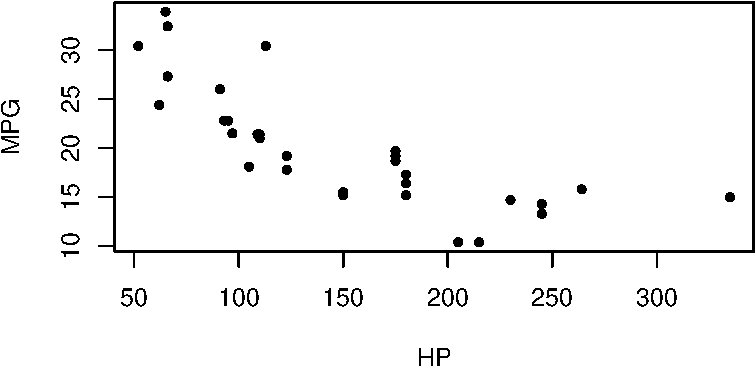
\includegraphics{index_files/figure-pdf/unnamed-chunk-3-1.pdf}

}

\end{figure}

\begin{Shaded}
\begin{Highlighting}[]
\NormalTok{model }\OtherTok{\textless{}{-}} \FunctionTok{lm}\NormalTok{(y}\SpecialCharTok{\textasciitilde{}}\NormalTok{x) }\CommentTok{\# This line of code creates a linear}
\CommentTok{\# regression model object in R. The response variable "y"}
\CommentTok{\# is modeled as a linear function of the predictor}
\CommentTok{\# variable "x". The syntax of the lm() function stands}
\CommentTok{\# for "linear model". After running this code, the object}
\CommentTok{\# model will contain information about the fit of the}
\CommentTok{\# regression model, such as the coefficients, residuals,}
\CommentTok{\# and other statistical properties.}

\FunctionTok{summary}\NormalTok{(model)}
\end{Highlighting}
\end{Shaded}

\begin{verbatim}

Call:
lm(formula = y ~ x)

Residuals:
    Min      1Q  Median      3Q     Max 
-5.7121 -2.1122 -0.8854  1.5819  8.2360 

Coefficients:
            Estimate Std. Error t value Pr(>|t|)    
(Intercept) 30.09886    1.63392  18.421  < 2e-16 ***
x           -0.06823    0.01012  -6.742 1.79e-07 ***
---
Signif. codes:  0 '***' 0.001 '**' 0.01 '*' 0.05 '.' 0.1 ' ' 1

Residual standard error: 3.863 on 30 degrees of freedom
Multiple R-squared:  0.6024,    Adjusted R-squared:  0.5892 
F-statistic: 45.46 on 1 and 30 DF,  p-value: 1.788e-07
\end{verbatim}

For the intercept this means that :

\begin{quote}
A ``hypothetical'' car with \texttt{hp\ =\ 0} will have
\texttt{mpg\ =\ 30.09} = \(\beta_0\)
\end{quote}

It's more interesting and instructive to consider the interpretation of
the slope:

Let's say we have some covariate \(x_0\) then the expected value for
\(y(x_0)\) is given by:

\[
y(x_0) = \beta_0 + \beta_1 x_0
\]

What's the expected value for \(x_0 + 1\)?

\[
\begin{align}
y(x_0 + 1) &= \beta_0 + \beta_1 \times (x_0 + 1)\\ \\
&= \beta_0 + \beta_1 x_0 + \beta_1\\ \\
&= y(x_0) + \beta_1\\ \\
\implies \beta_1 &= y(x_0 + 1) - y(x_0)
\end{align}
\]

\begin{center}\rule{0.5\linewidth}{0.5pt}\end{center}

\hypertarget{categorical-covariates}{%
\subsection{Categorical covariates}\label{categorical-covariates}}

Up until now, we have looked at \_simple\_ linear regression models
where both \(x\) and \(y\) are quantitative.

Let's confirm that \texttt{cyl} is indeed categorical:

\begin{Shaded}
\begin{Highlighting}[]
\NormalTok{mtcars}\SpecialCharTok{$}\NormalTok{cyl}
\end{Highlighting}
\end{Shaded}

\begin{verbatim}
 [1] 6 6 4 6 8 6 8 4 4 6 6 8 8 8 8 8 8 4 4 4 4 8 8 8 8 4 4 4 8 6 8 4
\end{verbatim}

Another example is with the iris dataset:

\begin{Shaded}
\begin{Highlighting}[]
\NormalTok{iris }\SpecialCharTok{\%\textgreater{}\%} \FunctionTok{head}\NormalTok{() }\SpecialCharTok{\%\textgreater{}\%} \FunctionTok{kable}\NormalTok{()}
\end{Highlighting}
\end{Shaded}

\begin{tabular}{r|r|r|r|l}
\hline
Sepal.Length & Sepal.Width & Petal.Length & Petal.Width & Species\\
\hline
5.1 & 3.5 & 1.4 & 0.2 & setosa\\
\hline
4.9 & 3.0 & 1.4 & 0.2 & setosa\\
\hline
4.7 & 3.2 & 1.3 & 0.2 & setosa\\
\hline
4.6 & 3.1 & 1.5 & 0.2 & setosa\\
\hline
5.0 & 3.6 & 1.4 & 0.2 & setosa\\
\hline
5.4 & 3.9 & 1.7 & 0.4 & setosa\\
\hline
\end{tabular}

Let's consider the following example:

We want to see if there is a relationship between \texttt{species} and
\texttt{sepal\ length}. How would we start the EDA?

\begin{Shaded}
\begin{Highlighting}[]
\NormalTok{y }\OtherTok{\textless{}{-}}\NormalTok{ iris}\SpecialCharTok{$}\NormalTok{Sepal.Length}
\NormalTok{x }\OtherTok{\textless{}{-}}\NormalTok{ iris}\SpecialCharTok{$}\NormalTok{Species}

\FunctionTok{boxplot}\NormalTok{(Sepal.Length }\SpecialCharTok{\textasciitilde{}}\NormalTok{ Species, iris)}
\end{Highlighting}
\end{Shaded}

\begin{figure}[H]

{\centering 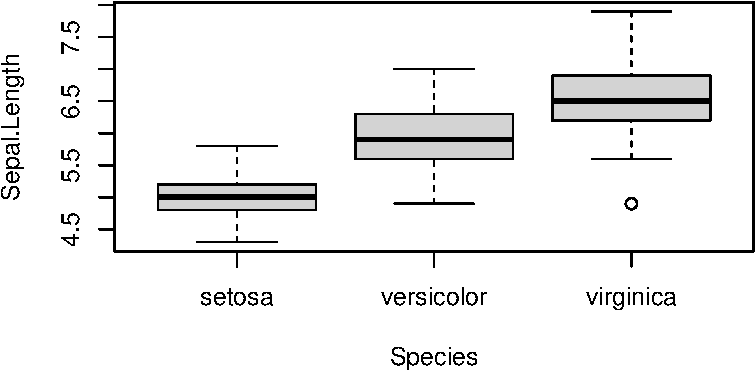
\includegraphics{index_files/figure-pdf/unnamed-chunk-6-1.pdf}

}

\end{figure}

Let's look just run a linear regression model and see what the model
output is going to look like:

\begin{Shaded}
\begin{Highlighting}[]
\NormalTok{cat\_model }\OtherTok{\textless{}{-}} \FunctionTok{lm}\NormalTok{(Sepal.Length }\SpecialCharTok{\textasciitilde{}}\NormalTok{ Species, iris)}
\NormalTok{cat\_model}
\end{Highlighting}
\end{Shaded}

\begin{verbatim}

Call:
lm(formula = Sepal.Length ~ Species, data = iris)

Coefficients:
      (Intercept)  Speciesversicolor   Speciesvirginica  
            5.006              0.930              1.582  
\end{verbatim}

Even if \(x\) is categorical, we can still write down the regression
model as follows:

\[
y_i = \beta_0 + \beta_1 x_i
\]

where \(x_i \in \{ setosa, \ versicolor, \ virginica \}\). This means
that we end up with , (fundamentally) three different models.

\begin{enumerate}
\def\labelenumi{\arabic{enumi}.}
\tightlist
\item
  \(y_i = \beta_0 + \beta_1 x_i =\) \texttt{setosa}
\item
  \(y_i = \beta_0 + \beta_1 x_i =\) \texttt{versicolor}
\item
  \(y_i = \beta_0 + \beta_1 x_i =\) \texttt{virginica}
\end{enumerate}

This implies that:

\begin{enumerate}
\def\labelenumi{\arabic{enumi}.}
\tightlist
\item
  \(y_i = \beta_0 + \beta_1 (x_i = c_1)\)
\item
  \(y_i = \beta_0 + \beta_1 (x_i = c_2)\)
\item
  \(y_i = \beta_0 + \beta_1 (x_i = c_3)\)
\end{enumerate}

This further implies that:

\begin{enumerate}
\def\labelenumi{\arabic{enumi}.}
\item
  \(y_i = \beta_0\)
\item
  \(y_i = \beta_0 + \beta_1 (x_i = c_2)\)
\item
  \(y_i = \beta_0 + \beta_1 (x_i = c_3)\)
\end{enumerate}

Now, the interpretation for the coefficients are as follows;

\hypertarget{intercept}{%
\paragraph{Intercept}\label{intercept}}

\(\beta_0\) is the expected \(y\) value when \(x\) belongs to the base
category. This is what the intercept is capturing.

\hypertarget{slopes}{%
\paragraph{Slopes}\label{slopes}}

\(\beta_1\) with the name \texttt{Species.versicolor} represents the
following:

\texttt{(Intercept)} = \(y(x = \texttt{setosa})\)

\texttt{Species.versicolor} =
\(y(x = \texttt{versicolor}) - y(x = \texttt{setosa})\)

\texttt{Species.virginica} =
\(y(x = \texttt{verginica}) - y(x = \texttt{setosa})\)

\hypertarget{reordering-the-factors}{%
\subsubsection{Reordering the factors}\label{reordering-the-factors}}

Let's say that we didn't want \texttt{setosa} to be the baseline level,
and, instead we wanted \texttt{virginica} to be the baseline level. How
would one do this?

First, we're going to reorder/relevel the categorical covariate

\begin{Shaded}
\begin{Highlighting}[]
\NormalTok{iris}\SpecialCharTok{$}\NormalTok{Species}
\end{Highlighting}
\end{Shaded}

\begin{verbatim}
  [1] setosa     setosa     setosa     setosa     setosa     setosa    
  [7] setosa     setosa     setosa     setosa     setosa     setosa    
 [13] setosa     setosa     setosa     setosa     setosa     setosa    
 [19] setosa     setosa     setosa     setosa     setosa     setosa    
 [25] setosa     setosa     setosa     setosa     setosa     setosa    
 [31] setosa     setosa     setosa     setosa     setosa     setosa    
 [37] setosa     setosa     setosa     setosa     setosa     setosa    
 [43] setosa     setosa     setosa     setosa     setosa     setosa    
 [49] setosa     setosa     versicolor versicolor versicolor versicolor
 [55] versicolor versicolor versicolor versicolor versicolor versicolor
 [61] versicolor versicolor versicolor versicolor versicolor versicolor
 [67] versicolor versicolor versicolor versicolor versicolor versicolor
 [73] versicolor versicolor versicolor versicolor versicolor versicolor
 [79] versicolor versicolor versicolor versicolor versicolor versicolor
 [85] versicolor versicolor versicolor versicolor versicolor versicolor
 [91] versicolor versicolor versicolor versicolor versicolor versicolor
 [97] versicolor versicolor versicolor versicolor virginica  virginica 
[103] virginica  virginica  virginica  virginica  virginica  virginica 
[109] virginica  virginica  virginica  virginica  virginica  virginica 
[115] virginica  virginica  virginica  virginica  virginica  virginica 
[121] virginica  virginica  virginica  virginica  virginica  virginica 
[127] virginica  virginica  virginica  virginica  virginica  virginica 
[133] virginica  virginica  virginica  virginica  virginica  virginica 
[139] virginica  virginica  virginica  virginica  virginica  virginica 
[145] virginica  virginica  virginica  virginica  virginica  virginica 
Levels: setosa versicolor virginica
\end{verbatim}

\begin{Shaded}
\begin{Highlighting}[]
\NormalTok{iris}\SpecialCharTok{$}\NormalTok{Species }\OtherTok{\textless{}{-}} \FunctionTok{relevel}\NormalTok{(iris}\SpecialCharTok{$}\NormalTok{Species, }\StringTok{"virginica"}\NormalTok{)}

\NormalTok{iris}\SpecialCharTok{$}\NormalTok{Species }\CommentTok{\# After}
\end{Highlighting}
\end{Shaded}

\begin{verbatim}
  [1] setosa     setosa     setosa     setosa     setosa     setosa    
  [7] setosa     setosa     setosa     setosa     setosa     setosa    
 [13] setosa     setosa     setosa     setosa     setosa     setosa    
 [19] setosa     setosa     setosa     setosa     setosa     setosa    
 [25] setosa     setosa     setosa     setosa     setosa     setosa    
 [31] setosa     setosa     setosa     setosa     setosa     setosa    
 [37] setosa     setosa     setosa     setosa     setosa     setosa    
 [43] setosa     setosa     setosa     setosa     setosa     setosa    
 [49] setosa     setosa     versicolor versicolor versicolor versicolor
 [55] versicolor versicolor versicolor versicolor versicolor versicolor
 [61] versicolor versicolor versicolor versicolor versicolor versicolor
 [67] versicolor versicolor versicolor versicolor versicolor versicolor
 [73] versicolor versicolor versicolor versicolor versicolor versicolor
 [79] versicolor versicolor versicolor versicolor versicolor versicolor
 [85] versicolor versicolor versicolor versicolor versicolor versicolor
 [91] versicolor versicolor versicolor versicolor versicolor versicolor
 [97] versicolor versicolor versicolor versicolor virginica  virginica 
[103] virginica  virginica  virginica  virginica  virginica  virginica 
[109] virginica  virginica  virginica  virginica  virginica  virginica 
[115] virginica  virginica  virginica  virginica  virginica  virginica 
[121] virginica  virginica  virginica  virginica  virginica  virginica 
[127] virginica  virginica  virginica  virginica  virginica  virginica 
[133] virginica  virginica  virginica  virginica  virginica  virginica 
[139] virginica  virginica  virginica  virginica  virginica  virginica 
[145] virginica  virginica  virginica  virginica  virginica  virginica 
Levels: virginica setosa versicolor
\end{verbatim}

Once we do the releveling, we can now run the regression model:

\begin{Shaded}
\begin{Highlighting}[]
\NormalTok{new\_cat\_model }\OtherTok{\textless{}{-}} \FunctionTok{lm}\NormalTok{(Sepal.Length }\SpecialCharTok{\textasciitilde{}}\NormalTok{ Species, iris)}
\NormalTok{new\_cat\_model}
\end{Highlighting}
\end{Shaded}

\begin{verbatim}

Call:
lm(formula = Sepal.Length ~ Species, data = iris)

Coefficients:
      (Intercept)      Speciessetosa  Speciesversicolor  
            6.588             -1.582             -0.652  
\end{verbatim}

\hypertarget{thursday-jan-19}{%
\subsection{Thursday, Jan 19}\label{thursday-jan-19}}

\begin{tcolorbox}[enhanced jigsaw, bottomrule=.15mm, coltitle=black, breakable, opacityback=0, rightrule=.15mm, colframe=quarto-callout-important-color-frame, toptitle=1mm, leftrule=.75mm, opacitybacktitle=0.6, bottomtitle=1mm, titlerule=0mm, title=\textcolor{quarto-callout-important-color}{\faExclamation}\hspace{0.5em}{TIL}, arc=.35mm, toprule=.15mm, colbacktitle=quarto-callout-important-color!10!white, colback=white, left=2mm]

Today, I learnt the following concepts in class:

\begin{enumerate}
\def\labelenumi{\arabic{enumi}.}
\tightlist
\item
  Multiple regression
\item
  Interpretation of coefficients of multiple regression
\item
  Significance of Interpretation of coefficients of multiple regression
\end{enumerate}

\end{tcolorbox}

Three plotting libraries

\begin{enumerate}
\def\labelenumi{\arabic{enumi}.}
\tightlist
\item
  base plot (plot)
\item
  ggplot
\item
  plotly
\end{enumerate}

\begin{Shaded}
\begin{Highlighting}[]
\FunctionTok{library}\NormalTok{(plotly)}
\end{Highlighting}
\end{Shaded}

\begin{verbatim}

Attaching package: 'plotly'
\end{verbatim}

\begin{verbatim}
The following object is masked from 'package:ggplot2':

    last_plot
\end{verbatim}

\begin{verbatim}
The following object is masked from 'package:stats':

    filter
\end{verbatim}

\begin{verbatim}
The following object is masked from 'package:graphics':

    layout
\end{verbatim}

\hypertarget{multiple-regression}{%
\subsubsection{Multiple Regression}\label{multiple-regression}}

This is the extension of simple linear regression to multiple covariates
\(X = [x_1 | x_2 | \dots |x_p]\), i.e.,

\[
y = \beta_0 + \beta_1 x_1 + \beta_2 x_2 + \dots \beta_p x_p + \epsilon
\]

In particular, the data looks like the following:

\textbar{} \(\mathbf y\) \textbar{} \(\mathbf x_1\) \textbar{}
\(\mathbf x_2\) \textbar{} \(\dots\) \textbar{} \(\mathbf x_p\)
\textbar{}

\textbar:-\/-\/-\/-\/-\/-\/-\/-\/-\textbar:-\/-\/-\/-\/-\/-\/-\/-\/-\textbar:-\/-\/-\/-\/-\/-\/-\/-\/-\textbar:-\/-\/-\/-\/-\/-\/-\/-\/-\textbar:-\/-\/-\/-\/-\/-\/-\/-\/-\textbar{}

\textbar{}\(y_{1}\) \textbar{}\(x_{1,1}\) \textbar{}\(x_{2,1}\)
\textbar{}\({...}\) \textbar{}\(x_{p,1}\) \textbar{}

\textbar{}\(y_{2}\) \textbar{}\(x_{1,2}\) \textbar{}\(x_{2,2}\)
\textbar{}\({...}\) \textbar{}\(x_{p,2}\) \textbar{}

\textbar{}\(y_{3}\) \textbar{}\(x_{1,3}\) \textbar{}\(x_{2,3}\)
\textbar{}\({…}\) \textbar{}\(x_{p,3}\) \textbar{}

\textbar{}\({\vdots}\) \textbar{}\({\vdots}\) \textbar{}\({\vdots}\)
\textbar{}\(\dots\) \textbar{}\(\dots\) \textbar{}\(\vdots\)

\textbar{}\(y_{n}\) \textbar{}\(x_{1,n}\) \textbar{}\(x_{2,n}\)
\textbar{}\({...}\) \textbar{}\(x_{p,n}\) \textbar{}

and, the full description of the model is as follows:

\[
y_i = \beta_0 + \beta_1 x_{1,i} + \beta_2 x_{2, i} + \dots + \beta_p x_{p,i} + \epsilon_i,
\]

knitr::kable()

\begin{quote}
In this, knitr is the package and kable() is the function.
\end{quote}

plotly::last\_plot()

\begin{quote}
In this, plotly is the package and last\_plot is the function.
\end{quote}

ggplot2::plot()

\begin{quote}
Similarly, in this ggplot2 is the package and plot() is the function.
\end{quote}

Consider the \texttt{Credit} dataset

\begin{Shaded}
\begin{Highlighting}[]
\FunctionTok{library}\NormalTok{(ISLR2)}
\FunctionTok{attach}\NormalTok{(Credit)}

\NormalTok{df }\OtherTok{\textless{}{-}}\NormalTok{ Credit }\SpecialCharTok{\%\textgreater{}\%} \FunctionTok{tibble}\NormalTok{()}
\FunctionTok{colnames}\NormalTok{(df) }\OtherTok{\textless{}{-}} \FunctionTok{tolower}\NormalTok{(}\FunctionTok{colnames}\NormalTok{(df))}
\NormalTok{df}
\end{Highlighting}
\end{Shaded}

\begin{verbatim}
# A tibble: 400 x 11
   income limit rating cards   age educat~1 own   student married region balance
    <dbl> <dbl>  <dbl> <dbl> <dbl>    <dbl> <fct> <fct>   <fct>   <fct>    <dbl>
 1   14.9  3606    283     2    34       11 No    No      Yes     South      333
 2  106.   6645    483     3    82       15 Yes   Yes     Yes     West       903
 3  105.   7075    514     4    71       11 No    No      No      West       580
 4  149.   9504    681     3    36       11 Yes   No      No      West       964
 5   55.9  4897    357     2    68       16 No    No      Yes     South      331
 6   80.2  8047    569     4    77       10 No    No      No      South     1151
 7   21.0  3388    259     2    37       12 Yes   No      No      East       203
 8   71.4  7114    512     2    87        9 No    No      No      West       872
 9   15.1  3300    266     5    66       13 Yes   No      No      South      279
10   71.1  6819    491     3    41       19 Yes   Yes     Yes     East      1350
# ... with 390 more rows, and abbreviated variable name 1: education
\end{verbatim}

and, we'll know at the following three columns: \texttt{income},
\texttt{rating}, \texttt{limit}.

\begin{Shaded}
\begin{Highlighting}[]
\NormalTok{df3 }\OtherTok{\textless{}{-}}\NormalTok{ df }\SpecialCharTok{\%\textgreater{}\%} \FunctionTok{select}\NormalTok{(income, rating, limit)}
\NormalTok{df3}
\end{Highlighting}
\end{Shaded}

\begin{verbatim}
# A tibble: 400 x 3
   income rating limit
    <dbl>  <dbl> <dbl>
 1   14.9    283  3606
 2  106.     483  6645
 3  105.     514  7075
 4  149.     681  9504
 5   55.9    357  4897
 6   80.2    569  8047
 7   21.0    259  3388
 8   71.4    512  7114
 9   15.1    266  3300
10   71.1    491  6819
# ... with 390 more rows
\end{verbatim}

If we want to see how the credit limit is related to income and credit
rating, we can visualize the following plot

\begin{Shaded}
\begin{Highlighting}[]
\NormalTok{fig }\OtherTok{\textless{}{-}} \FunctionTok{plot\_ly}\NormalTok{(df3, }\AttributeTok{x=}\SpecialCharTok{\textasciitilde{}}\NormalTok{income, }\AttributeTok{y=}\SpecialCharTok{\textasciitilde{}}\NormalTok{rating, }\AttributeTok{z=}\SpecialCharTok{\textasciitilde{}}\NormalTok{limit)}
\NormalTok{fig }\SpecialCharTok{\%\textgreater{}\%} \FunctionTok{add\_markers}\NormalTok{()}
\end{Highlighting}
\end{Shaded}

The regression mode is as follows:

\begin{Shaded}
\begin{Highlighting}[]
\NormalTok{model }\OtherTok{\textless{}{-}} \FunctionTok{lm}\NormalTok{(limit }\SpecialCharTok{\textasciitilde{}}\NormalTok{ income }\SpecialCharTok{+}\NormalTok{ rating, df3)}
\NormalTok{model}
\end{Highlighting}
\end{Shaded}

\begin{verbatim}

Call:
lm(formula = limit ~ income + rating, data = df3)

Coefficients:
(Intercept)       income       rating  
  -532.4711       0.5573      14.7711  
\end{verbatim}

What does the regression model look like here?

\begin{Shaded}
\begin{Highlighting}[]
\NormalTok{ranges }\OtherTok{\textless{}{-}}\NormalTok{ df3 }\SpecialCharTok{\%\textgreater{}\%}
    \FunctionTok{select}\NormalTok{(income, rating) }\SpecialCharTok{\%\textgreater{}\%}
    \FunctionTok{colnames}\NormalTok{() }\SpecialCharTok{\%\textgreater{}\%}
    \FunctionTok{map}\NormalTok{(\textbackslash{}(x) }\FunctionTok{seq}\NormalTok{(}\FloatTok{0.1} \SpecialCharTok{*} \FunctionTok{min}\NormalTok{(df3[x]), }\FloatTok{1.1} \SpecialCharTok{*} \FunctionTok{max}\NormalTok{(df3[x]),}
    \AttributeTok{length.out =} \DecValTok{50}\NormalTok{))}

\CommentTok{\# The code is generating a sequence of numbers that}
\CommentTok{\# represent the range of values for two variables income}
\CommentTok{\# and rating in the data frame df3. This sequence of}
\CommentTok{\# numbers is being stored in the ranges object.}
\CommentTok{\# The code uses the select function to select only the}
\CommentTok{\# columns income and rating from the data frame df3. Then}
\CommentTok{\# it uses the colnames function to extract the names of}
\CommentTok{\# these columns. Next, the code uses the map function}
\CommentTok{\# from the purrr package to apply a function to each}
\CommentTok{\# column name. The function generates a sequence of}
\CommentTok{\# numbers that covers the range of values in each column,}
\CommentTok{\# with a step of 0.1 times the minimum value and 1.1}
\CommentTok{\# times the maximum value. The number of numbers in the}
\CommentTok{\# sequence is specified by the length.out argument, which}
\CommentTok{\# is set to 50.}


\NormalTok{b }\OtherTok{\textless{}{-}}\NormalTok{ model}\SpecialCharTok{$}\NormalTok{coefficients }
\NormalTok{z }\OtherTok{\textless{}{-}} \FunctionTok{outer}\NormalTok{(}
\NormalTok{    ranges[[}\DecValTok{1}\NormalTok{]],}
\NormalTok{    ranges[[}\DecValTok{2}\NormalTok{]],}
    \FunctionTok{Vectorize}\NormalTok{(}\ControlFlowTok{function}\NormalTok{(x2, x3) \{}
\NormalTok{        b[}\DecValTok{1}\NormalTok{] }\SpecialCharTok{+}\NormalTok{ b[}\DecValTok{2}\NormalTok{] }\SpecialCharTok{*}\NormalTok{ x2 }\SpecialCharTok{+}\NormalTok{ b[}\DecValTok{3}\NormalTok{] }\SpecialCharTok{*}\NormalTok{ x3}
\NormalTok{    \})}
\NormalTok{)}

\CommentTok{\# This code is defining a matrix z that contains the}
\CommentTok{\# predicted values for a multiple linear regression model}
\CommentTok{\# with two predictors (income and rating) based on the}
\CommentTok{\# coefficients b from the model. The outer function}
\CommentTok{\# calculates the Cartesian product of the two ranges}
\CommentTok{\# (ranges[[1]] and ranges[[2]]), i.e., the values of x2}
\CommentTok{\# and x3 for all possible combinations of these two}
\CommentTok{\# variables. For each combination, the linear equation}
\CommentTok{\# represented by the coefficients b is calculated using}
\CommentTok{\# b[1] + b[2] * x2 + b[3] * x3 and the result is stored}
\CommentTok{\# in the matrix z.}


\NormalTok{fig }\SpecialCharTok{\%\textgreater{}\%} 
    \FunctionTok{add\_surface}\NormalTok{(}\AttributeTok{x =}\NormalTok{ ranges[[}\DecValTok{1}\NormalTok{]], }\AttributeTok{y =}\NormalTok{ ranges[[}\DecValTok{2}\NormalTok{]], }\AttributeTok{z =} \FunctionTok{t}\NormalTok{(z), }
    \AttributeTok{alpha =} \FloatTok{0.3}\NormalTok{) }\SpecialCharTok{\%\textgreater{}\%} 
    \FunctionTok{add\_markers}\NormalTok{()}
\end{Highlighting}
\end{Shaded}

\hypertarget{what-is-the-interpretation-for-this-coefficients}{%
\paragraph{What is the interpretation for this
coefficients?}\label{what-is-the-interpretation-for-this-coefficients}}

\begin{enumerate}
\def\labelenumi{\arabic{enumi}.}
\item
  \(\beta_0\) is the expected value of \(y\) when \(income = 0\) and
  \(rating = 0\)
\item
  \(\beta_1\) is saying that if \(rating\) is held constant and
  \(income\) changes by 1 unit, then the corresponding change in the
  \texttt{limit} is \(0.5573\).
\item
  \(\beta_2\) is saying that if \texttt{income} is held constant and
  \texttt{rating} changes by \(1\) unit, then the corresponding change
  in \texttt{limit} is \(14.771\).
\end{enumerate}

What about the significance ?

\begin{Shaded}
\begin{Highlighting}[]
\FunctionTok{summary}\NormalTok{(model)}
\end{Highlighting}
\end{Shaded}

\begin{verbatim}

Call:
lm(formula = limit ~ income + rating, data = df3)

Residuals:
    Min      1Q  Median      3Q     Max 
-420.97 -121.77   14.97  126.72  485.48 

Coefficients:
              Estimate Std. Error t value Pr(>|t|)    
(Intercept) -532.47115   24.17283 -22.028   <2e-16 ***
income         0.55727    0.42349   1.316    0.189    
rating        14.77115    0.09647 153.124   <2e-16 ***
---
Signif. codes:  0 '***' 0.001 '**' 0.01 '*' 0.05 '.' 0.1 ' ' 1

Residual standard error: 182.3 on 397 degrees of freedom
Multiple R-squared:  0.9938,    Adjusted R-squared:  0.9938 
F-statistic: 3.18e+04 on 2 and 397 DF,  p-value: < 2.2e-16
\end{verbatim}

\hypertarget{multiple-regression-1}{%
\subsubsection{Multiple regression}\label{multiple-regression-1}}

\begin{Shaded}
\begin{Highlighting}[]
\NormalTok{x }\OtherTok{\textless{}{-}} \FunctionTok{seq}\NormalTok{(}\DecValTok{0}\NormalTok{, }\DecValTok{1}\NormalTok{, }\AttributeTok{length.out =} \DecValTok{100}\NormalTok{)}
\NormalTok{b0 }\OtherTok{\textless{}{-}} \FloatTok{1.0}
\NormalTok{b1 }\OtherTok{\textless{}{-}} \FloatTok{2.0}
\NormalTok{y }\OtherTok{\textless{}{-}}\NormalTok{ b0 }\SpecialCharTok{+}\NormalTok{ b1 }\SpecialCharTok{*}\NormalTok{ x }\SpecialCharTok{+} \FunctionTok{rnorm}\NormalTok{(}\DecValTok{100}\NormalTok{) }\SpecialCharTok{*} \FloatTok{0.1}
\FunctionTok{plot}\NormalTok{(x,y, }\AttributeTok{pch =} \DecValTok{20}\NormalTok{)}
\end{Highlighting}
\end{Shaded}

\begin{figure}[H]

{\centering 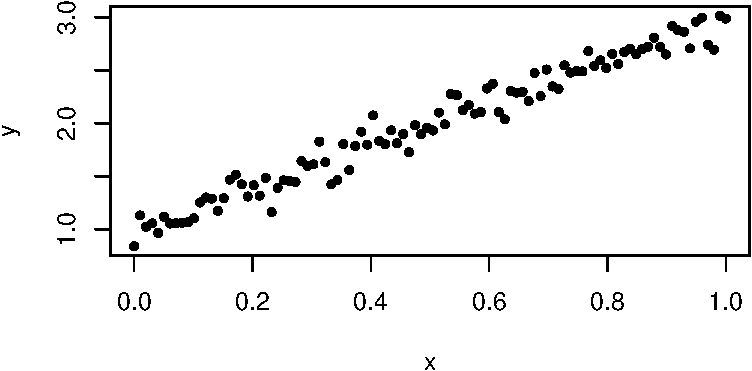
\includegraphics{index_files/figure-pdf/unnamed-chunk-17-1.pdf}

}

\end{figure}

\begin{Shaded}
\begin{Highlighting}[]
\NormalTok{model }\OtherTok{\textless{}{-}} \FunctionTok{lm}\NormalTok{(y}\SpecialCharTok{\textasciitilde{}}\NormalTok{x)}
\FunctionTok{summary}\NormalTok{(model)}
\end{Highlighting}
\end{Shaded}

\begin{verbatim}

Call:
lm(formula = y ~ x)

Residuals:
      Min        1Q    Median        3Q       Max 
-0.284198 -0.063344  0.006539  0.056224  0.281706 

Coefficients:
            Estimate Std. Error t value Pr(>|t|)    
(Intercept)  0.98138    0.02144   45.78   <2e-16 ***
x            2.00838    0.03704   54.22   <2e-16 ***
---
Signif. codes:  0 '***' 0.001 '**' 0.01 '*' 0.05 '.' 0.1 ' ' 1

Residual standard error: 0.108 on 98 degrees of freedom
Multiple R-squared:  0.9677,    Adjusted R-squared:  0.9674 
F-statistic:  2940 on 1 and 98 DF,  p-value: < 2.2e-16
\end{verbatim}

This code generates a linear model in R. It starts by generating an
\textbf{\texttt{x}} sequence of 100 equally spaced values between 0 and
1. Then it creates two variables, \textbf{\texttt{b0}} and
\textbf{\texttt{b1}}, with values of 1.0 and 2.0, respectively. It uses
these values to generate \textbf{\texttt{y}} with a formula
\textbf{\texttt{b0\ +\ b1\ *\ x\ +\ rnorm(100)\ *\ 0.7}}.
\textbf{\texttt{rnorm(100)}} generates random normal deviates with a
mean of 0 and standard deviation of 0.7. The code then plots
\textbf{\texttt{x}} against \textbf{\texttt{y}} using the
\textbf{\texttt{plot()}} function and fits a linear regression model to
the data using the \textbf{\texttt{lm()}} function with the formula
\textbf{\texttt{y\ \textasciitilde{}\ x}}. Finally, it summarizes the
results of the linear regression model using the
\textbf{\texttt{summary()}} function.

The value \textbf{\texttt{0.1}} in the code is the standard deviation of
the normal distribution used to generate random noise to add to the
\textbf{\texttt{y}} variable.

\texttt{As\ the\ standard\ deviation\ increases,\ the\ Adjusted\ R-squared\ decreases}

\begin{Shaded}
\begin{Highlighting}[]
\FunctionTok{library}\NormalTok{(ISLR2)}
\FunctionTok{library}\NormalTok{(dplyr)}
\FunctionTok{library}\NormalTok{(ggplot2)}

\FunctionTok{attach}\NormalTok{(ISLR2}\SpecialCharTok{::}\NormalTok{Credit)}
\end{Highlighting}
\end{Shaded}

\begin{verbatim}
The following objects are masked from Credit:

    Age, Balance, Cards, Education, Income, Limit, Married, Own,
    Rating, Region, Student
\end{verbatim}

\begin{Shaded}
\begin{Highlighting}[]
\NormalTok{df }\OtherTok{\textless{}{-}}\NormalTok{ Credit }\SpecialCharTok{\%\textgreater{}\%} \FunctionTok{tibble}\NormalTok{() }\SpecialCharTok{\%\textgreater{}\%} \FunctionTok{rename\_all}\NormalTok{(tolower)}
\NormalTok{df}
\end{Highlighting}
\end{Shaded}

\begin{verbatim}
# A tibble: 400 x 11
   income limit rating cards   age educat~1 own   student married region balance
    <dbl> <dbl>  <dbl> <dbl> <dbl>    <dbl> <fct> <fct>   <fct>   <fct>    <dbl>
 1   14.9  3606    283     2    34       11 No    No      Yes     South      333
 2  106.   6645    483     3    82       15 Yes   Yes     Yes     West       903
 3  105.   7075    514     4    71       11 No    No      No      West       580
 4  149.   9504    681     3    36       11 Yes   No      No      West       964
 5   55.9  4897    357     2    68       16 No    No      Yes     South      331
 6   80.2  8047    569     4    77       10 No    No      No      South     1151
 7   21.0  3388    259     2    37       12 Yes   No      No      East       203
 8   71.4  7114    512     2    87        9 No    No      No      West       872
 9   15.1  3300    266     5    66       13 Yes   No      No      South      279
10   71.1  6819    491     3    41       19 Yes   Yes     Yes     East      1350
# ... with 390 more rows, and abbreviated variable name 1: education
\end{verbatim}

\begin{Shaded}
\begin{Highlighting}[]
\NormalTok{model }\OtherTok{\textless{}{-}} \FunctionTok{lm}\NormalTok{(limit }\SpecialCharTok{\textasciitilde{}}\NormalTok{ rating }\SpecialCharTok{+}\NormalTok{ married, df)}
\NormalTok{model}
\end{Highlighting}
\end{Shaded}

\begin{verbatim}

Call:
lm(formula = limit ~ rating + married, data = df)

Coefficients:
(Intercept)       rating   marriedYes  
    -528.09        14.87       -25.97  
\end{verbatim}

\begin{Shaded}
\begin{Highlighting}[]
\FunctionTok{ggplot}\NormalTok{(df) }\SpecialCharTok{+} 
      \FunctionTok{geom\_point}\NormalTok{(}\FunctionTok{aes}\NormalTok{(}\AttributeTok{x =}\NormalTok{ rating, }\AttributeTok{y =}\NormalTok{ limit, }\AttributeTok{color =}\NormalTok{ married)) }\SpecialCharTok{+}
      \FunctionTok{geom\_point}\NormalTok{(}\FunctionTok{aes}\NormalTok{(}\AttributeTok{x =}\NormalTok{ rating, }\AttributeTok{y =}\NormalTok{ limit, }\AttributeTok{fill=}\NormalTok{ married))}
\end{Highlighting}
\end{Shaded}

\begin{figure}[H]

{\centering 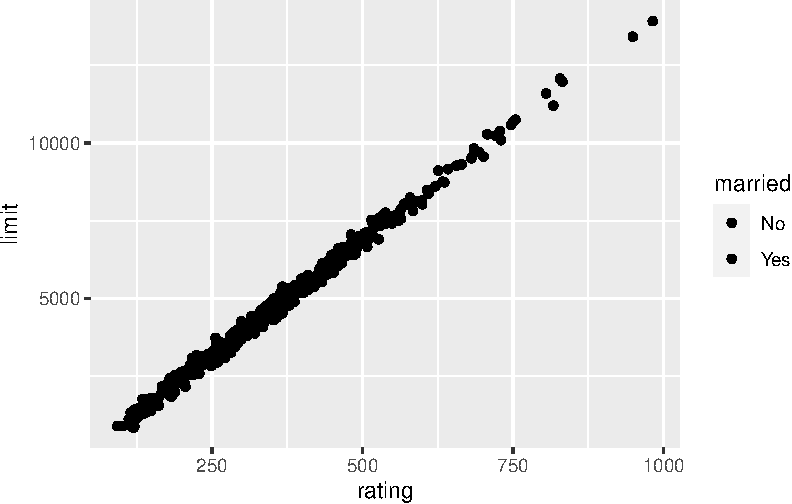
\includegraphics{index_files/figure-pdf/unnamed-chunk-18-1.pdf}

}

\end{figure}

This code is loading the \textbf{\texttt{ISLR2}} and
\textbf{\texttt{dplyr}} packages, as well as the
\textbf{\texttt{ggplot2}} library. The \textbf{\texttt{Credit}} data set
is loaded from the \textbf{\texttt{ISLR2}} package and saved as a tibble
named \textbf{\texttt{df}}. \textbf{\texttt{attach}} is a function in R
that temporarily loads a data set into the search path, so that its
objects can be accessed directly by name, rather than having to
reference the data set each time with its full name. In other words, you
can use the variables in the data set as if they are in the workspace.
However, it is generally not recommended to use \textbf{\texttt{attach}}
as it can lead to naming conflicts and make the code harder to
maintain.The \textbf{\texttt{rename\_all}} function is used to convert
the names of all columns in the tibble to lowercase. A linear regression
model is then fit to the data using the formula
\textbf{\texttt{limit\ \textasciitilde{}\ rating\ +\ married}}. The
response variable \textbf{\texttt{limit}} is modeled as a linear
function of the predictor variables \textbf{\texttt{rating}} and
\textbf{\texttt{married}}. Finally, a scatterplot is created using
\textbf{\texttt{ggplot2}}, with the points colored and filled according
to the value of the \textbf{\texttt{married}} variable.



\end{document}
